\subsection{Méthodologie de développement logiciel embarqué STM32}

Le séquenceur et l'expérience APEX reposent tous deux sur des microcontrôleurs de la famille STM32, développés au moyen des
outils fournis par STMicroelectronics. Avant de détailler le fonctionnement logiciel propre à chacun de ces deux systèmes,
cette section présente les principes généraux qui structurent leur développement : l'environnement de génération de code
STM32Cube, l'organisation du dépôt logiciel, et les deux paradigmes d'exécution employés sur le projet.

\subsubsection{Le framework STM32Cube et la couche d'abstraction matérielle (\acrshort{HAL})}

Bien que les membres de l'association soient globalement plus familiers de la programmation Arduino et de l'utilisation de
pilotes (\textit{drivers}) de capteurs multiplateformes disponibles en ligne, il a été décidé de privilégier STM32Cube et la
\acrshort{HAL}, avec des pilotes développés en interne plutôt que des bibliothèques tierces.\\

Là où l'écosystème Arduino repose sur des cartes de développement prêtes à l'emploi, associées à un environnement qui prend en
charge l'essentiel de la configuration du microcontrôleur, l'approche STM32 part du composant lui-même. STMicroelectronics
propose une large gamme de microcontrôleurs, déclinés en séries aux ressources et aux performances très variées, et met à
disposition un ensemble d'outils logiciels, regroupés sous le nom de STM32Cube, destinés à les configurer et à les programmer.
Cet ensemble comprend notamment un outil de configuration graphique, STM32CubeMX, et un ensemble de bibliothèques
d'abstraction du matériel, dont la \acrfull{HAL}.\\

STM32CubeMX permet de définir, pour un microcontrôleur donné, l'affectation des broches, l'arborescence d'horloges ainsi que la
configuration des périphériques internes (minuteries, liaisons \acrshort{UART}, bus \acrshort{I2C}, etc.), puis de générer
automatiquement le code d'initialisation correspondant. Ce code prend la forme de fonctions dédiées, une par périphérique
configuré (par exemple \texttt{MX\_USART1\_UART\_Init}), appelées séquentiellement au démarrage du programme.

\begin{figure}[H]
    \centering
    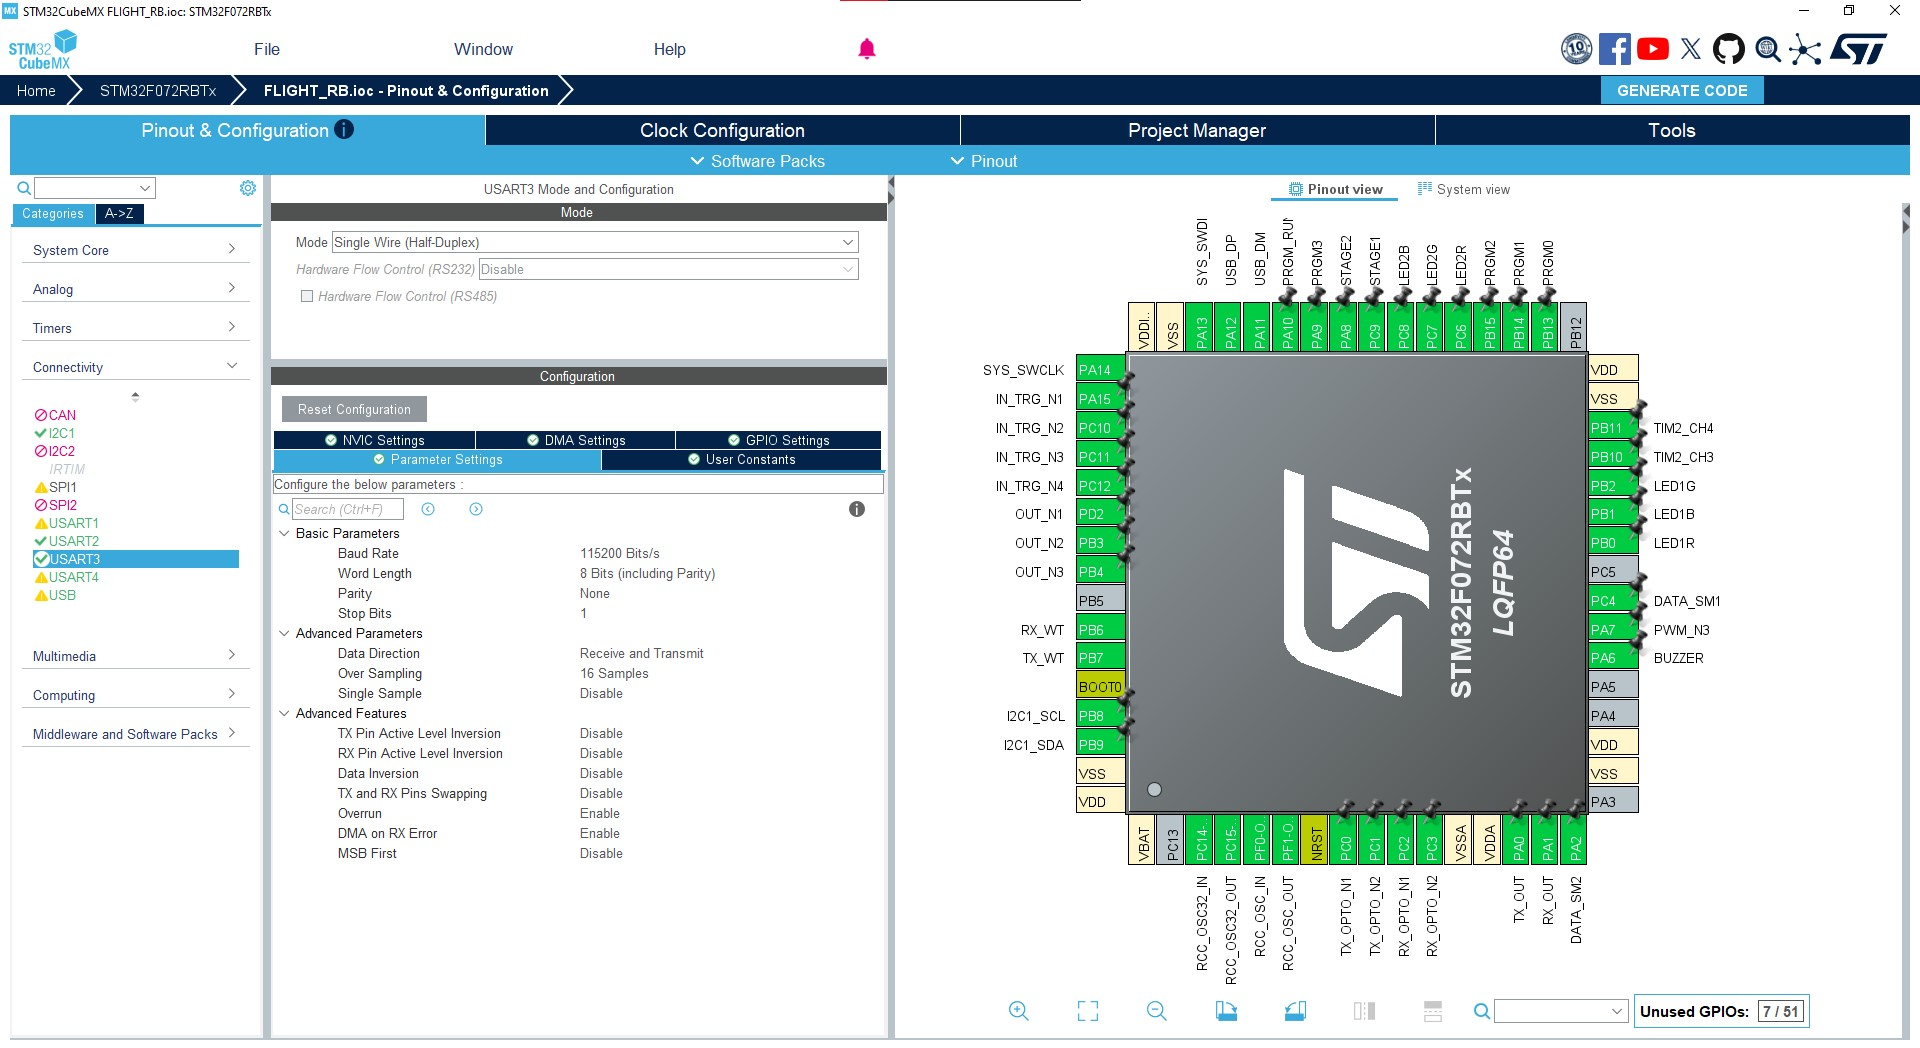
\includegraphics[width=0.85\textwidth]{figures/elec/STM32CubeMX_1.jpg}
    \caption{Configuration d'un bus UART avec STM32CubeMX}
\end{figure}

Par ailleurs, un microcontrôleur STM32 ne dispose pas d'une fréquence de fonctionnement unique et figée. A partir d'une source
primaire (oscillateur interne ou quartz externe), un ensemble de multiplicateurs et de diviseurs permet d'établir la fréquence
du c\oe{}ur, puis celles des différents bus internes auxquels sont rattachés les périphériques. C'est de cette arborescence que
découlent, entre autres, la période des minuteries, la vitesse des liaisons série et celle des bus de communication. Un réglage
inadapté ne se traduit généralement pas par une erreur de compilation, mais par un comportement temporel erroné à l'exécution,
ce qui rend sa vérification d'autant plus importante. STM32CubeMX en propose une représentation graphique complète, dans laquelle chaque
fréquence intermédiaire est affichée et contrôlée vis-à-vis des limites du composant.

\begin{figure}[H]
    \centering
    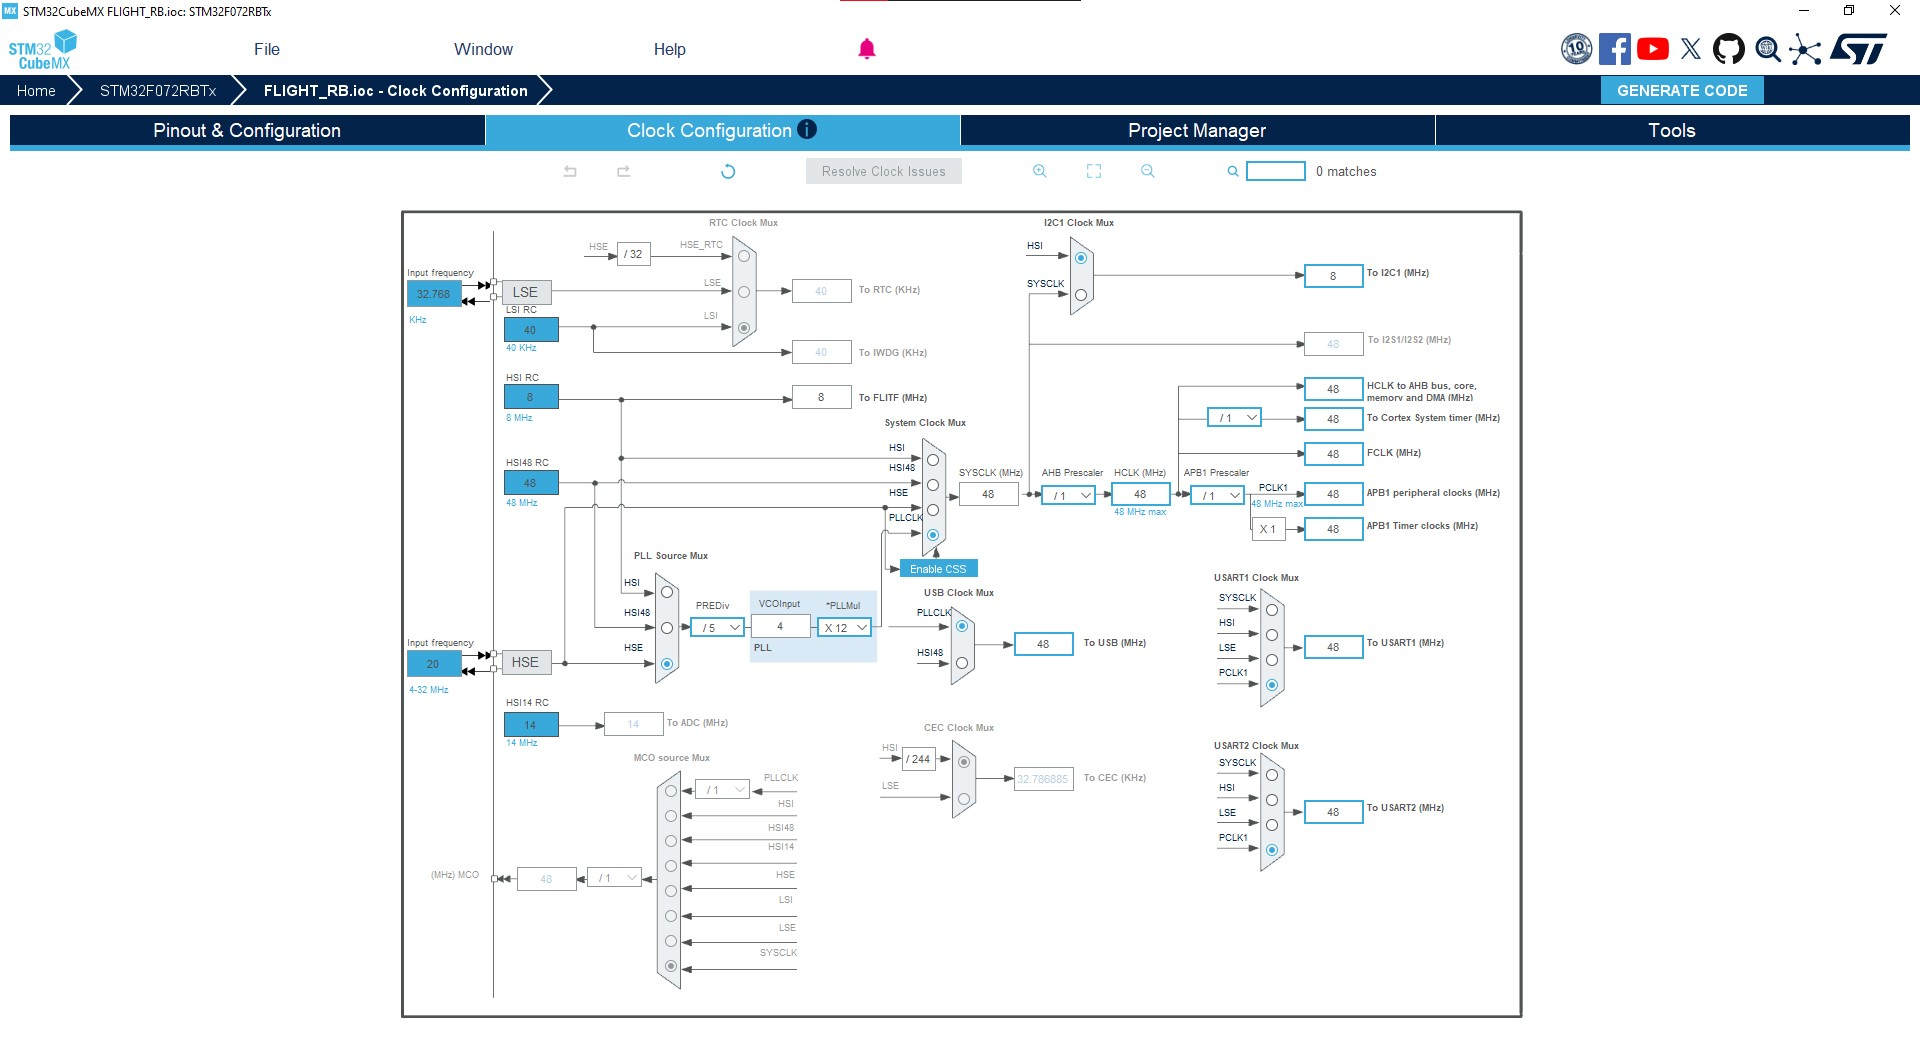
\includegraphics[width=0.85\textwidth]{figures/elec/STM32CubeMX_2.jpg}
    \caption{Configuration d'horloges avec STM32CubeMX}
\end{figure}

Cette étape de configuration n'a pas d'équivalent dans le monde Arduino, où elle est réalisée implicitement par le framework.
L'abstraction y est poussée au point de masquer largement l'architecture sous-jacente : un même programme peut être compilé
presque à l'identique pour une carte à base d'AVR ou pour un ESP32. Sur STM32, la cible compte réellement, et son paramétrage
représente un travail supplémentaire, en contrepartie duquel l'intégralité du comportement du composant reste visible et
modifiable.\\

Le code d'initialisation produit par STM32CubeMX s'appuie quant à lui sur la \acrfull{HAL}, une bibliothèque logicielle qui
expose une interface de programmation (\acrshort{API}) unifiée pour piloter les périphériques du microcontrôleur
(\texttt{HAL\_GPIO\_WritePin}, \texttt{HAL\_UART\_Transmit}, \texttt{HAL\_I2C\_Master\_Receive}, etc.), sans que le développeur
ait à manipuler directement les registres internes du composant. Son rôle est comparable à celui que joue le framework Arduino
avec des fonctions telles que \texttt{digitalWrite} ou \texttt{Serial.print}, mais elle se situe à un niveau nettement plus
proche du matériel : chaque fonction agit sur un périphérique explicitement identifié et préalablement configuré, et son effet
sur les registres reste directement traçable dans le code source fourni. Cette proximité se traduit également par un code
exécutable plus léger et plus prévisible : là où une écriture sur une broche traverse, côté Arduino, plusieurs tables de
correspondance et vérifications avant d'atteindre le registre concerné, l'équivalent \acrshort{HAL} se réduit à quelques
instructions. Le surcoût ne provient pas du compilateur, identique dans les deux cas, mais du nombre de couches d'abstraction
traversées à l'exécution. Dans un domaine aussi exigeant que l'aérospatial, pouvoir estimer ce que devient réellement une ligne
de code une fois compilée constitue un critère de choix à part entière.\\

L'\acrshort{API} unifiée de la \acrshort{HAL} permet par ailleurs de transposer un même code applicatif d'une série STM32 à une
autre. Cette transposition reste toutefois conditionnée au maintien d'une configuration matérielle explicite, propre à chaque
cible : la \acrshort{HAL} masque les registres, pas le microcontrôleur. Les pilotes développés en interne viennent se greffer
au-dessus de cette couche : ce sont eux qui portent la logique propre à chaque composant externe, en s'appuyant sur les fonctions
de la \acrshort{HAL} pour les échanges bas niveau.

\newpage

L'écosystème Arduino (Arduino Nano, ESP32, framework Arduino) répond quant à lui à des besoins différents, et conserve des
atouts réels pour un projet associatif : une prise en main rapide, une abondance de bibliothèques déjà écrites pour la
quasi-totalité des capteurs et actionneurs du commerce, et donc un temps de développement initial très court. Piloter un
servomoteur ou une centrale inertielle s'y résume souvent à quelques appels de fonction. Ces qualités ont cependant une
contrepartie : ces bibliothèques sont conçues pour un usage générique, sans garantie sur leur comportement temporel (fonctions
bloquantes non documentées, boucles d'attente actives...) ni sur la qualité de leur implémentation, et leur fonctionnement
interne reste, pour l'essentiel, une boîte noire pour qui les utilise. Le constat s'étend au-delà du seul comportement temporel :
la configuration des ressources partagées entre plusieurs composants y est généralement figée par défaut et jamais exposée au
développeur, de sorte que dès que plusieurs composants aux besoins différents doivent cohabiter sur une même ressource (un bus
de données \acrshort{SPI} par exemple), ce réglage implicite devient difficile à ajuster, voire à diagnostiquer en cas de
conflit. Ces inconnues sont difficilement compatibles avec un système impliquant la sécurité du vol, où le comportement de
chaque fonction exécutée doit pouvoir être vérifié.\\
 
Le choix de pilotes \og maison \fg{} répond à ces limites. Chaque pilote (servomoteurs STS, centrale inertielle WT901B, LED,
buzzer...) et chaque utilitaire logiciel (tampon circulaire, messagerie interne par abonnement, planification d'animations
LED...) a été écrit au sein de l'équipe, au-dessus de la \acrshort{HAL}. Aucune ligne de code exécutée en vol ne provient ainsi
d'une source dont le comportement n'a pas été établi, ce qui rend possible l'audit du budget temporel de chaque fonction
appelée. \\
 
Ce choix répond également à une volonté de développement de compétences techniques personnelles. Configurer soi-même sa cible
oblige à en comprendre le fonctionnement interne, et l'écriture puis la validation de ses propres pilotes constituent, dans le
même esprit, un objectif d'apprentissage à part entière en programmation comme en électronique numérique bas niveau,
complémentaire à la réalisation du projet lui-même.\\
 
Cette approche a toutefois un coût. Le développement de chaque pilote et de chaque utilitaire depuis zéro demande un temps bien
supérieur à l'intégration d'une bibliothèque existante, sans bénéficier de la robustesse qu'apporte un usage et une correction
communautaires étalés dans le temps : chaque bogue rencontré doit être identifié et corrigé en interne, sans retour d'expérience
extérieur. Elle alourdit également l'intégration de nouveaux membres au sein de l'association, moins familiers d'un développement
bas niveau que du monde Arduino, et fait reposer l'intégralité de la maintenance du code sur quelques développeurs.

\newpage

\subsubsection{Organisation du dépôt : \texttt{Core}, \texttt{UserProjects} et \texttt{UserLibraries}}

Le développement de plusieurs cartes distinctes, chacune donnant lieu à un programme de vol et à une série de programmes de
test, impose une organisation de dépôt répondant à trois besoins :\\
\begin{itemize}
    \item Transposer facilement une bibliothèque écrite en interne d'un projet STM32Cube à un autre, sans avoir à la réécrire ni
    à l'extraire manuellement de son contexte d'origine. Par exemple, le séquenceur et l'expérience APEX utilisent tous deux le
    capteur \texttt{WT901B} et donc disposent d'un driver commun.\\
    \item Assurer la traçabilité de l'ensemble des tests menés au fil du développement itératif du code : chaque programme de
    test écrit à une étape donnée reste présent dans le dépôt et reste exécutable par la suite.\\
    \item Pouvoir passer très rapidement d'un programme à un autre, afin de conduire des tests de non-régression sans
    manipulation lourde.\\
\end{itemize}
L'arborescence retenue, commune aux deux systèmes STM32 du projet, repose sur trois répertoires principaux : \texttt{Core},
\texttt{UserProjects} et \texttt{UserLibraries}.

% \vspace{0.6cm}
\vfill

\hspace*{-\parindent}%
\begin{minipage}{0.5\textwidth}
    \paragraph*{\textbf{\texttt{Core} --}} Le répertoire \texttt{Core} contient le code généré par STM32CubeMX : initialisation
    des horloges et des périphériques, gestionnaires d'interruption, ainsi qu'un fichier \texttt{main.c} volontairement minimal.
    Outre les en-têtes générés décrivant les périphériques configurés (\texttt{main.h}, \texttt{gpio.h}, \texttt{tim.h},
    \texttt{usart.h}, \texttt{i2c.h}, \texttt{dma.h}, ...), ce dernier n'inclut qu'un seul en-tête applicatif,
    \texttt{project.h}, qui déclare deux fonctions : \texttt{setup()}, appelée une fois le matériel initialisé, et
    \texttt{loop()}, appelée à chaque itération de la boucle infinie qui suit.\\
     
    Ce \og main générique \fg{} ne contient aucune logique applicative. Il constitue un point d'entrée neutre, identique quel
    que soit le programme réellement exécuté par la carte, et n'a plus à être modifié une fois la configuration matérielle
    établie. La structure \texttt{setup()}/\texttt{loop()} reprend volontairement celle du framework Arduino, familière à
    l'ensemble des membres de l'association.
\end{minipage}
\hfill
\begin{minipage}{0.35\textwidth}
    \begin{lstlisting}[language=C, frame=tb]
#include "main.h"
#include "gpio.h"
...

#include "project.h"

int main(void) {
    HAL_Init();
    SystemClock_Config();
    MX_GPIO_Init();
    MX_I2C1_Init();
    ...

    setup();
    while (1) {
        loop();
    }
}
    \end{lstlisting}
\end{minipage}
\hfill\hfill

% \vspace{0.6cm}
\vfill

\hfill
\hspace*{-\parindent}%
\begin{minipage}{0.25\textwidth}
    \begin{lstlisting}[language=C, frame=tb]
// project.c

void setup() {
    ...
}
    
void loop() {
    ...
}
    \end{lstlisting}
\end{minipage}
\hfill
\begin{minipage}{0.65\textwidth}
    \paragraph*{\textbf{\texttt{UserProjects} --}} Le fichier \texttt{project.h} inclus par le \texttt{main} et son implémentation
    \texttt{project.c} appartiennent au répertoire \texttt{UserProjects}. Celui-ci regroupe, sous forme d'un sous-dossier par
    programme, l'ensemble des firmwares développés au cours du projet : le programme de vol (\texttt{full\_seq}), ses variantes
    par étage (\texttt{full\_seq\_stage\_1}, \texttt{full\_seq\_stage\_2}), ainsi qu'une série de programmes de test dédiés à la
    validation isolée d'un sous-système (\texttt{test\_servo}, \texttt{test\_uart}, \texttt{test\_wt901b}, \texttt{test\_ihf},
    \texttt{test\_buzzer}, etc.). Chaque sous-dossier possède ainsi ses propres \texttt{project.h} et \texttt{project.c}, et
    donc sa propre implémentation de \texttt{setup()} et \texttt{loop()}.\\
\end{minipage}

Cette organisation sert directement les deux derniers besoins évoqués plus haut. Plutôt que d'intégrer d'emblée l'ensemble des
sous-systèmes (servomoteurs, centrale inertielle, mise à feu, interface homme-fusée...) dans un unique programme complexe,
chacun a pu être développé et éprouvé indépendamment dans un firmware dédié, réduisant d'autant la surface d'erreur au moment de
l'intégration finale. Ces programmes n'étant jamais supprimés, ils constituent un historique exécutable des validations menées :
en cas de dysfonctionnement ou après une modification d'une bibliothèque partagée, il reste possible de reprendre un
sous-système isolément sans avoir à interpréter le comportement du programme complet.

% \vfill

\newpage

\setlength{\DTbaselineskip}{7pt}
% \DTsetlength{0.2em}{0.5em}{0.1em}{0.4pt}{1.6pt}

\begin{minipage}{0.5\textwidth}
    \paragraph*{\textbf{\texttt{UserLibraries} --}} Le troisième répertoire, \texttt{UserLibraries}, rassemble le code partagé
    entre ces programmes. Il se divise lui-même en deux familles. Le sous-répertoire \texttt{drivers} contient les pilotes
    propres à un composant matériel donné (\texttt{STS} pour les servomoteurs, \texttt{WT901B} pour la centrale inertielle,
    \texttt{led}, \texttt{buzzer}), tandis que \texttt{utils} regroupe les utilitaires indépendants du matériel
    (\texttt{circular\_buffer}, \texttt{data\_topic}, \texttt{led\_scheduler}, \texttt{actuator}, \texttt{quaternion},
    \texttt{iir\_filter}, \texttt{waveform}...). Chaque bibliothèque étant autonome et rassemblée dans un dossier unique, elle
    peut être employée par n'importe quel programme du dépôt, et transposée telle quelle vers un autre projet STM32Cube en
    recopiant ce seul dossier et en déclarant ses chemins dans la configuration de compilation. Une correction apportée à une
    bibliothèque bénéficie par ailleurs immédiatement à l'ensemble des firmwares qui l'utilisent.\\

    Chaque module, qu'il s'agisse d'une bibliothèque ou d'un projet, suit la même arborescence interne : un dossier
    \texttt{Core/Inc} pour les en-têtes et un dossier \texttt{Core/Src} pour les sources. Les premiers sont déclarés comme
    chemins d'inclusion et les seconds comme fichiers à compiler, de sorte que n'importe quel fichier du projet peut inclure un
    en-tête par son seul nom, sans avoir à exprimer un chemin relatif dépendant de sa propre position dans l'arborescence.
\end{minipage}
\hfill
\begin{minipage}{0.40\textwidth}
    \vspace{-0.8cm}
    \begin{figure}[H]
        \scriptsize\dirtree{%
        .1 ....
        .1 Core.
            .2 Inc.
                .3 gpio.h.
                .3 i2c.h.
                .3 ....
                .3 main.h.
            .2 Src.
                .3 gpio.c.
                .3 i2c.c.
                .3 ....
                .3 main.c.
        .1 UserProjects.
            .2 project\_0.
                .3 Inc.
                    .4 project.h.
                .3 Src.
                    .4 project.c.
            .2 ....
        .1 UserLibraries.
            .2 drivers.
                .3 sx127x.
                    .4 Core.
                        .5 Inc.
                            .6 sx127x.h.
                            .6 sx127x\_common.h.
                            .6 sx127x\_fsk\_ook.h.
                            .6 sx127x\_lora.h.
                        .5 Src.
                            .6 sx127x.c.
                            .6 sx127x\_common.c.
                            .6 sx127x\_fsk\_ook.c.
                            .6 sx127x\_lora.c.
                .3 ....
            .2 utils.
                .3 data\_topic.
                    .4 Core.
                        .5 Inc.
                            .6 data\_topic.h.
                        .5 Src.
                            .6 data\_topic.c.
                .3 ....
        .1 ....
        }
        \caption{Arborescence d'un dépôt logiciel type utilisé pour le séquenceur et l'expérience APEX}
    \end{figure}
\end{minipage}
\hfill\hfill


\begin{minipage}{0.55\textwidth}  
    \begin{figure}[H]
        \centering
        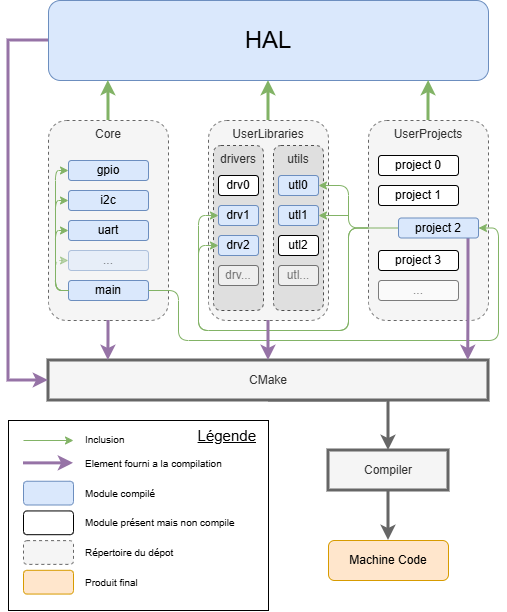
\includegraphics[width=\textwidth]{figures/elec/chaine_compilation_stm32.drawio.png}
        \caption{Chaîne de compilation d'un dépôt logiciel type du projet}
    \end{figure}
\end{minipage}
\hfill
\begin{minipage}{0.35\textwidth}
    La sélection du programme à compiler s'opère enfin au niveau de la configuration CMake, par l'intermédiaire d'une variable
    \texttt{CMAKE\_USER\_PROJECT\_PATH} désignant le sous-dossier de \texttt{UserProjects} retenu. Cette variable est ensuite
    utilisée pour compléter la liste des chemins d'inclusion et celle des fichiers sources, si bien que l'ajout d'un nouveau
    programme ne demande que la création d'un sous-dossier respectant la convention \texttt{Core/Inc} et \texttt{Core/Src}. Les
    autres chemins restent présents dans le fichier de configuration sous forme de lignes commentées : basculer d'un programme
    à l'autre revient à déplacer un commentaire, sans modification du reste du dépôt.
    \vfill\vfill
\end{minipage}

\newpage

\subsubsection{Boucle séquentielle et système d'exploitation temps réel}

Au-delà de cette organisation commune, le séquenceur et l'expérience APEX diffèrent sur un point structurant : le modèle
d'exécution retenu pour la boucle \texttt{loop()}.\\


\begin{minipage}{0.30\textwidth}
    \begin{figure}[H]
        \centering
        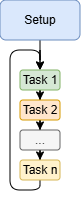
\includegraphics[width=0.4\textwidth]{figures/elec/superloop.drawio.png}
        \caption{Boucle séquentielle (superloop)}
    \end{figure}
\end{minipage}
\hfill
\begin{minipage}{0.60\textwidth}
Le séquenceur repose sur une architecture dite en boucle séquentielle (ou superloop) : à chaque itération, \texttt{loop()}
exécute successivement une série de fonctions \og pas à pas \fg, chacune non bloquante, qui font avancer l'état du système d'une
petite quantité avant de rendre la main. Il n'existe qu'un seul flux d'exécution, sans ordonnanceur ni préemption : le programme
fait exactement ce que son code décrit, dans l'ordre où il le décrit. Cette simplicité a une contrepartie stricte : aucune
fonction appelée dans la boucle ne doit bloquer plus de quelques centaines de microsecondes, sous peine de retarder l'ensemble
des autres tâches du système. Le budget de temps d'exécution de chaque fonction doit donc être audité individuellement.
\end{minipage}

\vspace{0.4cm}

Cette contrainte a une conséquence structurelle sur la manière d'écrire le code. Une tâche qui, écrite naturellement,
s'exprimerait de façon linéaire (par exemple envoyer une commande, attendre une réponse, traiter la réponse) doit être découpée
en étapes élémentaires réparties sur plusieurs itérations de la boucle. La majeure partie du temps chaque tâche doit être
réécrite sous forme de machine à états, et tout ce qui constituerait normalement le contexte local de la fonction doit être
conservé explicitement dans des variables d'état persistantes entre les appels.\\

Tant que les tâches sont peu nombreuses et simples, ce coût reste modeste. Il croît en revanche rapidement avec le nombre de
tâches concurrentes et le nombre d'étapes de chacune : la liste des variables à maintenir s'allonge, et les machines à états
deviennent difficiles à faire évoluer sans risque de régression. C'est précisément lorsque cette complexité devient
prépondérante que le recours à un système d'exploitation temps réel prend tout son sens : celui-ci fournit nativement les
mécanismes de sauvegarde et de restauration de contexte que la boucle séquentielle impose d'écrire à la main.\\

\begin{minipage}{0.55\textwidth}
L'expérience APEX repose quant à elle sur un système d'exploitation temps réel (\acrshort{RTOS}), en l'occurrence FreeRTOS. Le
programme y est découpé en plusieurs tâches, ordonnancées de manière préemptive par le noyau de l'OS, chacune pouvant se mettre
en attente (sur un délai, une donnée à recevoir, une ressource partagée) sans bloquer l'exécution des autres tâches. Chaque
tâche disposant de sa propre pile, son contexte est sauvegardé et restauré automatiquement à chaque commutation : le code peut
donc rester écrit de manière linéaire, sans machine à états ni variables d'état explicites.
\end{minipage}
\hfill
\begin{minipage}{0.35\textwidth}
    \begin{figure}[H]
        \centering
        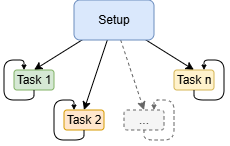
\includegraphics[width=\textwidth]{figures/elec/rtos.drawio.png}
        \caption{Système d'exploitation temps réel (RTOS)}
    \end{figure}
\end{minipage}

\vspace{0.4cm}

Cette architecture facilite le développement de systèmes devant gérer plusieurs flux simultanés et faiblement synchronisés entre
eux, au prix d'une complexité supplémentaire, déplacée ailleurs : protection des ressources partagées entre tâches,
dimensionnement de la pile de chacune, et une garantie de déterminisme temporel global plus difficile à établir que sur une
boucle séquentielle unique.\\

Le choix de l'un ou l'autre paradigme sur chaque système découle directement de leurs contraintes respectives : le séquenceur,
soumis à des exigences fortes de sûreté de vol et de déterminisme temporel, retient la boucle séquentielle ; l'expérience APEX,
qui doit gérer en parallèle l'acquisition de plusieurs capteurs, deux protocoles de télémesure et la communication avec le
séquenceur, retient FreeRTOS.

\newpage
